\section{An\'alisis 1: La Universidad Rusa de la Amistad de los Pueblos (URAP)}
Vamos a realizar un an\'alisis de nuestro traceroute sobre "La Universidad Rusa de la Amistad de los Pueblos (URAP)". Es una universidad que se encuentra en Rusia, en la ciudad de Mosc\'u.\newline

El host de dicha universidad es http://www.rudn.ru/ (IP: 193.232.218.50).\\	

\subsection{Par\'ametros de entrada}
\begin{itemize}
\item Host: www.rudn.ru
\item Tiempo Limite: 2
\item Cant. Iteraciones en cada nodo: 10
\item Recorrido m\'aximo de nodos: 30 (TTL m\'aximo)
\item alpha: 0.05
\end{itemize}
El tiempo limite indica cuanto esperar de respuesta, como m\'aximo, a un nodo.\newline

\subsection{Resultados obtenidos}

Captura general de los resultados obtenidos:

\begin{figure}[h]
	%\begin{center}
    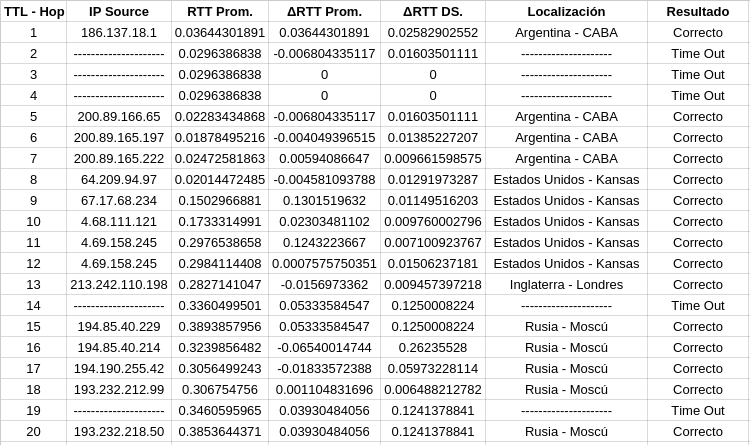
\includegraphics[width=1\textwidth]{img_analisis1/tabla.png}
     %\label{fig:ICMPlista} 
	%\end{center} 
    
\end{figure}
\vspace{0.25cm}


De la muestra obtuvimos una distribuci\'on Normal, y los siguientes enlaces significativos (submarinos):
\begin{itemize}
\item Hop 9
\item Hop 11
\item Hop 16
\end{itemize}

\subsubsection{Gr\'afico en mapa}

\begin{figure}[h]
	%\begin{center}
    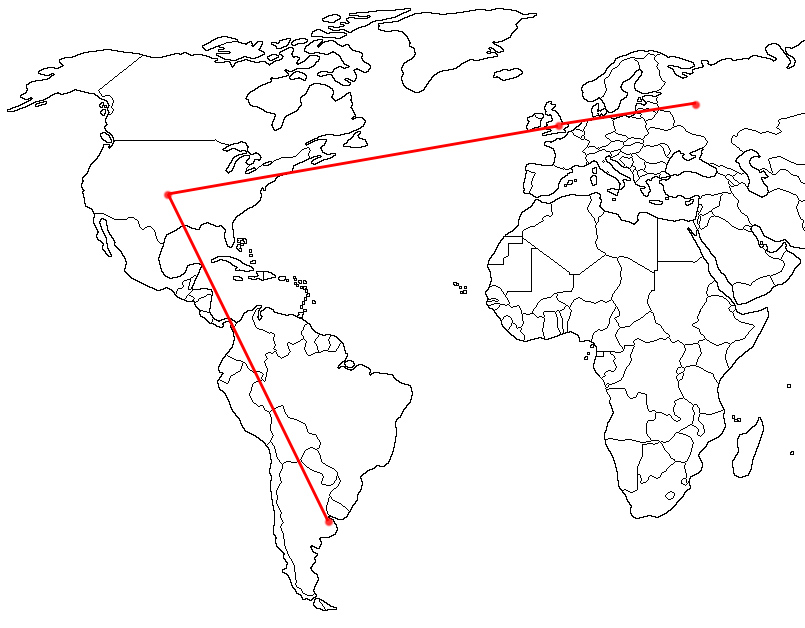
\includegraphics[width=0.8\textwidth]{img_analisis1/mapa.jpg}
     %\label{fig:ICMPlista} 
	%\end{center} 
    
\end{figure}
\vspace{0.25cm}


\subsection{An\'alisis de la captura obtenida}

Mirando la tabla presentada uno podr\'ia estimar que los saltos m\'as significativos (enlaces submarinos) estar\'an dados por aquellos que tengan una distancia bastante grande con respecto a su enlace anterior. A simple vistas, estas deber\'ian situarse en los siguientes saltos, dado que pasan de un continente a otro:
\begin{itemize}
\item Del Hop 7 al Hop 8, dado que pasa de Argentina a Estados Unidos.
\item Del Hop 12 al Hop 13, dado que pasa de Estados Unidos a Inglaterra.
\item Del Hop 13 al Hop 15, dado que pasa de Inglaterra a Rusia.
\end{itemize}

\begin{figure}[h]
	%\begin{center}
    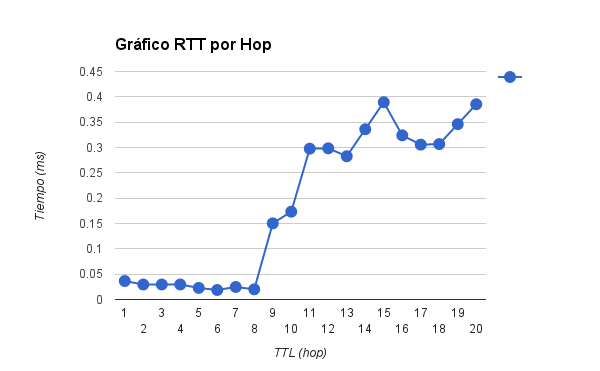
\includegraphics[width=0.65\textwidth]{img_analisis1/rtt_hop.png}
     %\label{fig:ICMPlista} 
	%\end{center} 
    
\end{figure}
\vspace{0.25cm}

Del gr\'afico se aprecian grandes subidas entre los siguientes saltos:
\begin{itemize}
\item Del Hop 8 al Hop 9.
\item Del Hop 10 al Hop 11.
\item Del Hop 13 al Hop 15. Cabe mencionar que esta diferencia es atenuada por nuestra forma de resolver el time out (interpolando entre el 13 y el 15) del Hop 14.
\item Del Hop 18 al Hop 20. Se vuelve a presentar el mismo caso que el item anterior.
\end{itemize}
De la misma manera podemos notar un franco descendente entre el Hop 15 y 16.

\begin{figure}[h]
	%\begin{center}
    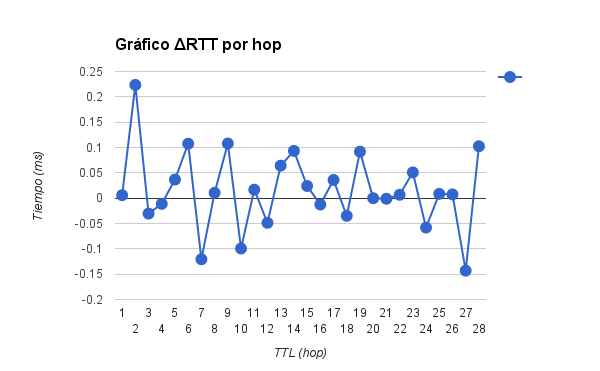
\includegraphics[width=0.65\textwidth]{img_analisis1/delta_rtt_hop.png}
     %\label{fig:ICMPlista} 
	%\end{center} 
    
\end{figure}
\vspace{0.25cm}
Observando el gr\'afico podemos apreciar la tardanza, para bien o para mal, de ese enlace en particular, olvidandonos del resto de los enlaces por los que la traza pas\'o. Habiendo mencionado esto, los Hop m\'as significativos fueron los siguientes:
\begin{itemize}
\item Hop 9 y Hop 11. Como podemos ver, lo que tardan en responder estos enlaces es significativamente alto con respecto a los dem\'as.
\item En menor medida tenemos los Hops 14 y 15, muy parecidos a los 19 y 20. Podemos no considerar a los Hops 14 y 19, dado que fueron productos de dos time outs y su valor no es del todo real.
\item Tambi\'en obtuvimos un enlace, el Hop 16, que respondi\'o bastante m\'as r\'apido que los dem\'as, dado que su resultado es bastante m\'as bajo que el resto.
\end{itemize}

\begin{figure}[h]
	%\begin{center}
    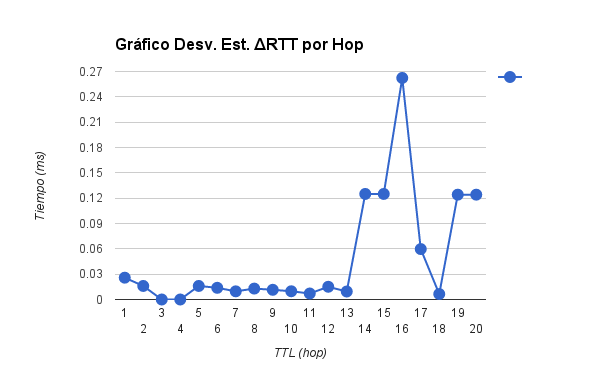
\includegraphics[width=0.65\textwidth]{img_analisis1/ds_delta_rtt_hop.png}
     %\label{fig:ICMPlista} 
	%\end{center} 
    
\end{figure}
\vspace{0.25cm}

En este paso hablaremos del \'ultimo de los gr\'aficos. Cabe mencionar que el desv\'io estandar nos indica que tan dispersos son los datos que nos llegaron de nuestra muestra. Como el \'analisis lo vamos a hacer sobre $\Delta$RTT, vamos a obtener, sobre cada enlace, que tan alejado de la media estuvieron los datos que nos aportaron. El an\'alisis de los datos son los siguientes:
\begin{itemize}
\item Podemos ver que los valores vienen manteniendose constantes hasta el Hop 13, dandonos una idea de que cada enlace constenta mas o menos en un tiempo acorde. 
\item El Hop 16 es el que presenta el desvio estandar m\'as elevado.
\item En menor medida tenemos los Hops 15 y 20 sucede algo similiar, sin tomar en cuenta a los Hops 14 y 19.
\item Otro que sobresale de los dem\'as es el hop 17, sin ser un valor demasiado grande.
\end{itemize}

%\cleardoublepage


\subsection{An\'alisis de los enlaces m\'as relevantes}
\begin{itemize}
\item Hop 8 y 13: Si bien era esperable que estos enlaces fueran marcados como un enlaces significativos, dado que pasan de Argentina a Estados Unidos y de Estados Unidos a Inglaterra, sus respuestas de paquetes ICMP fueron significativamente r\'apidas con respecto a la de sus nodos antecesores.
\item Hop 9 y 11: Fueron indicados como un enlaces submarinos (significativos), y gran parte de eso se debe a su demora en responder mensajes ICMP. Descartamos el caso de una congesti\'on grande inst\'antanea, dado que no presentaron valores grandes en el desv\'io estandar.
\item Hop 13: Otro enlace que estimamos que podr\'ia haber sido marcado como enlace significativo, dado que pasa de Estados Unidos a Inglaterra. Sin embargo, esto fue atenuado porque sus antecesores respond\'ian considerablemente m\'as lento.
\item Hop 15: Era un candidato tanto como 8 y 13, y de hecho marc\'o bastante trascendencia en los resultados analizados. No lleg\'o a quedar marcada como enlace significativo por la atenuaci\'on del time out del Hop 14.
\item Hop 16: Marcado como enlace significativo. Lo raro de este enlace es que super\'o el tests de grubbs debido a que su respuesta fue mucho m\'as r\'apida que su antecesor, como se puede apreciar en el gr\'afico $\Delta$RTT. Viendo los resultados del gr\'afico correspondiente al desv\'io estandar, se puede observar que los resultados fueron muy dispersos por lo que podemos asumir que responde muy r\'apido en algunos momentos particulares, o que quiz\'as algunos tiempos se calcularon erroneamente. Otra de las cosas que pudimos asumir, es que quizas, en algunos momentos, dicho enlace estaba completamente descongestionado, con lo cual respond\'ia los paquetes mucho m\'as r\'apido su antecesor. 
\item Hop 20: Este enlace, de no haber sido por el time out del Hop 19, podr\'ia haber sido considerado como un enlace significativo. No tiene mucho sentido dado que su enlace antecesor est\'a en Mosc\'u junto a \'el. Pero si miramos los resultados obtenido, vemos que este enlace es bastante inestable con respecto a su antecesor y responde de forma m\'as lenta (lo contrario al Hop 16), lo que origina su relevancia en el an\'alisis.
\end{itemize}

\subsection{Conclusi\'on}
Al iniciar la investigaci\'on, uno estima que los resultados de los enlaces m\'as relevantes, con m\'as demoras o menos demoras, estar\'an dados por aquellos con mayor o menor distancias f\'isica; principalmente cuando se tienen que comunicar de un continente a otro con respecto a comunicaciones del mismo pa\'is. Sin embargo, en este \'analisis, se observa que ese no es el \'unico par\'ametro significativo. Si bien a medida que la distancia entre enlaces se agranda, el tiempo generalmente aumenta, se pudo observar que los tiempos de cada enlace se deben tambi\'en en gran parte a como est\'en configurados, el tr\'afico de datos que tenga en ese momento (congesti\'on), la velocidad con la que contestan a dicha petici\'on, la manera que resolvemos cuando hay enlaces que no contestan, etc.